\documentclass[border=10pt]{standalone}
\usepackage{tikz}
\usetikzlibrary{arrows.meta, shadows.blur, backgrounds, calc, decorations.pathmorphing}
\usepackage{amsmath}
\begin{document}
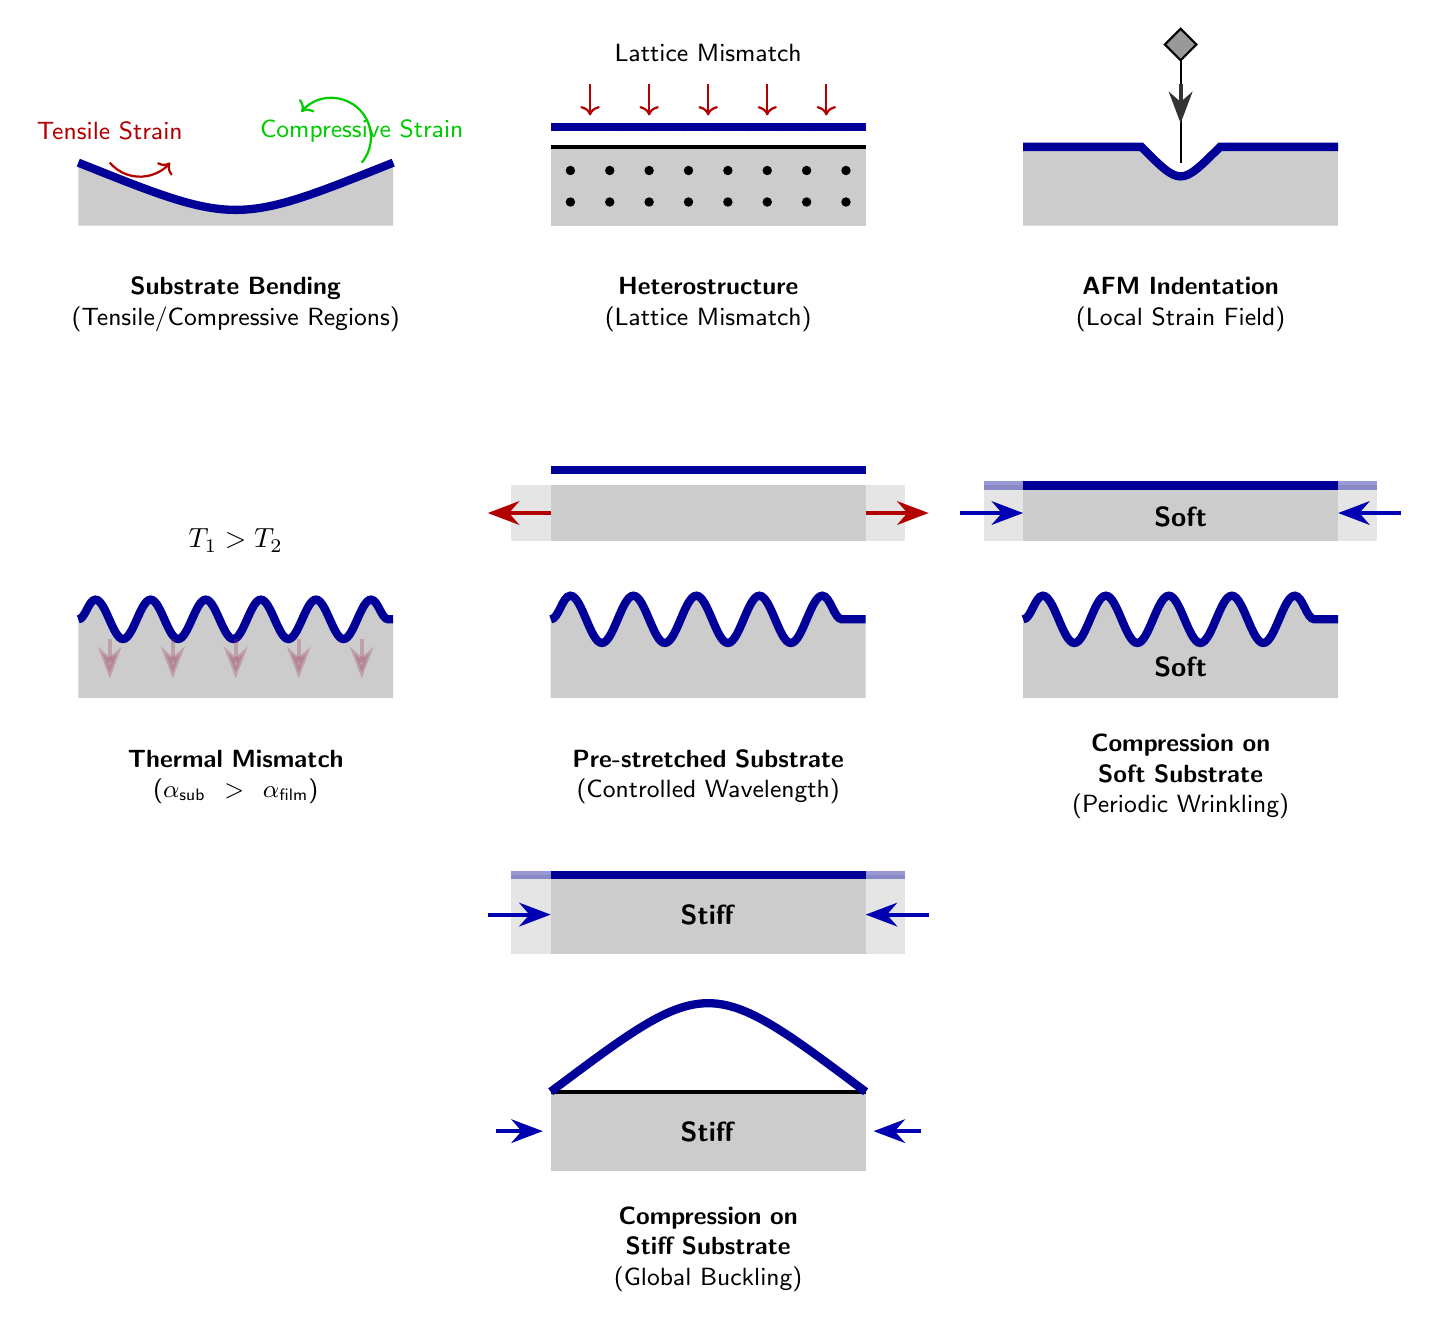
\begin{tikzpicture}[font=\sffamily\bfseries]

  % Define updated styles
  \tikzset{
    substrate/.style={fill=gray!40},
    topline/.style={draw=black, line width=1.5pt},
    tmd/.style={line width=3pt, blue!60!black},
    arrow/.style args={#1}{-{Stealth[length=4mm,width=3mm]},line width=1.5pt,color=#1},
    panel label/.style={font=\sffamily\small,align=center,text width=4.2cm},
    title/.style={font=\sffamily\bfseries\large}
  }

% ---------- Top Row ----------

%% Panel 1: Substrate Bending
\begin{scope}[shift={(-6,6)}]
  % Substrate shape with bend
  \fill[substrate]
    (-2,-0.7) .. controls (0,-1.5) .. (2,-0.7)
    -- (2,-1.5) -- (-2,-1.5) -- cycle;

  % Blue arc line for TMD
  \draw[tmd]
    (-2,-0.7) .. controls (0,-1.5) .. (2,-0.7);

  % Curved tensile arrow (left side)
  \draw[->, thick, red!70!black]
    ([shift={(0,0.2)}] -1.6,-0.9) arc[start angle=220, end angle=320, radius=0.5];
  \node[font=\sffamily\small, red!70!black] at (-1.6,-0.3) {Tensile Strain};

  % Curved compressive arrow (right side)
  \draw[->, thick, green!80!black]
    ([shift={(0,0.2)}] 1.6,-0.9) arc[start angle=-40, end angle=140, radius=0.5];
  \node[font=\sffamily\small, green!80!black] at (1.6,-0.3) {Compressive Strain};

  % Panel label
  \node[panel label] at (0,-2.5) 
    {\textbf{Substrate Bending}\\(Tensile/Compressive Regions)};
\end{scope}

%% Panel 2: Heterostructure Lattice Mismatch
\begin{scope}[shift={(0,6)}]
  % Substrate
  \fill[substrate] (-2,-1.5) rectangle (2,-0.5);
  \draw[topline] (-2,-0.5) -- (2,-0.5);
  
  % TMD layer
  \draw[tmd] (-2,-0.25) -- (2,-0.25);
  
  % Lattice visualization for substrate (larger spacing)
  \foreach \x in {-1.75,-1.25,...,1.75} {
    \fill[black] (\x,-0.8) circle (0.06);
    \fill[black] (\x,-1.2) circle (0.06);
  }
  
  % Lattice visualization for TMD (smaller spacing)
  \foreach \x in {-1.9,-1.5,...,1.9} {
    \fill[blue!60!black] (\x,-0.25) circle (0.05);
  }
  
  % Strain arrows pointing down
  \foreach \x in {-1.5,-0.75,0,0.75,1.5} {
    \draw[->, thick, red!70!black] (\x,0.3) -- (\x,-0.1);
  }
  
  % Label for mismatch
  \node[font=\sffamily\small] at (0,0.7) {Lattice Mismatch};
  
  % Panel label
  \node[panel label] at (0,-2.5)
    {\textbf{Heterostructure}\\(Lattice Mismatch)};
\end{scope}

%% Panel 3: AFM Indentation
\begin{scope}[shift={(6,6)}]
  % Substrate with indentation
  \path[substrate]
    (-2,-0.5) -- (-0.5,-0.5)
    .. controls (0,-1) .. (0.5,-0.5) -- (2,-0.5)
    -- (2,-1.5) -- (-2,-1.5) -- cycle;

  % Indentation line
  \draw[tmd]
    (-2,-0.5) -- (-0.5,-0.5)
    .. controls (0,-1) .. (0.5,-0.5) -- (2,-0.5);

  % AFM probe tip stem and force arrow
  \draw[thick] (0,0.6) -- (0,-0.7);
  \draw[arrow=black!80] (0,0.3) -- (0,-0.2);

  % AFM tip
  \draw[fill=black!40, draw=black, thick] 
    (0,1) -- (-0.2,0.8) -- (0,0.6) -- (0.2,0.8) -- cycle;

  % Panel label
  \node[panel label] at (0,-2.5)
    {\textbf{AFM Indentation}\\(Local Strain Field)};
\end{scope}

% ---------- Middle Row ----------

%% Panel 4: Thermal Mismatch
\begin{scope}[shift={(-6,0)}]
  \path[substrate]
    (-2,-0.5)
    decorate[decoration={snake, amplitude=0.25cm, segment length=0.7cm}]
      { -- (2,-0.5) }
    -- (2,-1.5) -- (-2,-1.5) -- cycle;

  \draw[tmd]
    (-2,-0.5)
    decorate[decoration={snake, amplitude=0.25cm, segment length=0.7cm}]
      { -- (2,-0.5) };

  % Temperature label
  \node at (0,0.5) {$T_1 > T_2$};

  % Compression arrows
  \foreach \x in {-1.6,-0.8,...,1.6}
    \draw[arrow=purple!50!gray, opacity=0.3] (\x,-0.75) -- (\x,-1.25);

  % Panel label
  \node[panel label] at (0,-2.5)
    {\textbf{Thermal Mismatch}\\($\alpha_{\text{sub}} > \alpha_{\text{film}}$)};
\end{scope}

%% Panel 5: Pre-Stretch/Release with vertically stacked scenarios and updated arrow style
\begin{scope}[shift={(0,0.9)}]
  % First scene: Stretched state (top)
  \begin{scope}[yshift=0.6cm]
    % Stretched substrate
    \fill[substrate, opacity=0.5] (-2.5,-1) rectangle (2.5,-0.3);   
    % Stretching arrows (red, pointing outward) - moved even farther apart
    \draw[arrow=red!70!black] (-1.5,-0.65) -- (-2.8,-0.65);
    \draw[arrow=red!70!black] (1.5,-0.65) -- (2.8,-0.65);    
    \fill[substrate] (-2,-1) rectangle (2,-0.3);   
    % TMD layer (flat)

    \draw[tmd] (-2,-0.1) -- (2,-0.1);

    

  \end{scope}
  
  % Second scene: Released state with ripples - better aligned with row
  \begin{scope}[yshift=-0.9cm]
    % Relaxed substrate
    \path[substrate]
      (-2,-0.5)
      decorate[decoration={snake, amplitude=0.3cm, segment length=0.8cm}]
        { -- (2,-0.5) }
      -- (2,-1.5) -- (-2,-1.5) -- cycle;

    % TMD layer with ripples
    \draw[tmd]
      (-2,-0.5)
      decorate[decoration={snake, amplitude=0.3cm, segment length=0.8cm}]
        { -- (2,-0.5) };
  \end{scope}
  
  % Panel label
  \node[panel label] at (0,-3.4)
    {\textbf{Pre-stretched Substrate}\\(Controlled Wavelength)};
\end{scope}

%% Panel 6: Compression on Stiff Substrate (Global Buckling)


\begin{scope}[shift={(6,0)}]

  \begin{scope}[yshift=1.5cm]
    % Stretched substrate
    \fill[substrate, opacity=0.5] (-2.5,-1) rectangle (2.5,-0.3);   
    \draw[tmd,opacity=0.4] (-2.5,-0.3) -- (2.5,-0.3);    
    % Stretching arrows (red, pointing outward) - moved even farther apart
    \draw[arrow=blue!70!black] (-2.8,-0.65) -- (-2,-0.65);
    \draw[arrow=blue!70!black] (2.8,-0.65) -- (2,-0.65);    
    \fill[substrate] (-2,-1) rectangle (2,-0.3);   
    % TMD layer (flat)

    \draw[tmd] (-2,-0.3) -- (2,-0.3);

      \node at (0,-0.7) {\textbf{Soft}};


  \end{scope}
  
  \path[substrate]
    (-2,-0.5)
    decorate[decoration={snake, amplitude=0.3cm, segment length=0.8cm}]
      { -- (2,-0.5) }
    -- (2,-1.5) -- (-2,-1.5) -- cycle;

  \draw[tmd]
    (-2,-0.5)
    decorate[decoration={snake, amplitude=0.3cm, segment length=0.8cm}]
      { -- (2,-0.5) };

  \node at (0,-1.1) {\textbf{Soft}};

  \node[panel label] at (0,-2.5)
    {\textbf{Compression on Soft Substrate}\\(Periodic Wrinkling)};  
\end{scope}

% ---------- Bottom Row ----------

% Empty panel for left position
\begin{scope}[shift={(-6,-6.2)}]
  % Intentionally left empty
\end{scope}

%% Panel 7: Compression on Soft Substrate (Periodic Wrinkling) - moved to center
\begin{scope}[shift={(0,-6)}]

  \begin{scope}[yshift=2.25cm]
    % Stretched substrate
    \fill[substrate, opacity=0.5] (-2.5,-1) rectangle (2.5,0);   
    \draw[tmd,opacity=0.4] (-2.5,0) -- (2.5,0);    
    % Stretching arrows (red, pointing outward) - moved even farther apart
    \draw[arrow=blue!70!black] (-2.8,-0.5) -- (-2,-0.5);
    \draw[arrow=blue!70!black] (2.8,-0.5) -- (2,-0.5);    
    \fill[substrate] (-2,-1) rectangle (2,0);   
    % TMD layer (flat)

    \draw[tmd] (-2,0) -- (2,0);

   \node at (0,-0.5) {\textbf{Stiff}};
   

  \end{scope}
  
  \fill[substrate] (-2,-0.5) rectangle (2,-1.5);
  \draw[topline] (-2,-0.5) -- (2,-0.5);
  \draw[tmd] (-2,-0.5) .. controls (0,1) .. (2,-0.5);
  \draw[arrow=blue!70!black] (-2.7,-1) -- (-2.1,-1);
  \draw[arrow=blue!70!black] (2.7,-1) -- (2.1,-1);

  % Label inside substrate
  \node at (0,-1.01) {\textbf{Stiff}};

  \node[panel label] at (0,-2.5)
    {\textbf{Compression on Stiff Substrate}\\(Global Buckling)};
\end{scope}

% Empty panel for right position
\begin{scope}[shift={(6,-6)}]
  % Intentionally left empty
\end{scope}

\end{tikzpicture}
\end{document}
